\documentclass[a4paper]{article}
\usepackage{natbib}
\usepackage{url}
\usepackage{hyperref}
\hypersetup{
    colorlinks,
    citecolor=black,
    filecolor=black,
    linkcolor=black,
    urlcolor=black,
	linktoc=all,
	bookmarksdepth=paragraph
}
\usepackage[cyr]{aeguill}
\usepackage[utf8]{inputenc}
\usepackage[francais]{babel}
\usepackage{amsmath}
\usepackage{graphicx}
\usepackage{parskip}
\usepackage{fancyhdr}
\usepackage{listings}

%%configuration de listings
\lstset{
	language=PHP,
	basicstyle=\ttfamily\footnotesize, %
	identifierstyle=\color{red}, %
	keywordstyle=\bfseries\color{blue}, %
	stringstyle=\color{black!60}, %
	commentstyle=\color{green!95!yellow!1}, %
	columns=flexible, %
	tabsize=2, %
	extendedchars=true, %
	showspaces=false, %
	showstringspaces=false, %
	numbers=left, %
	numberstyle=\tiny, %
	breaklines=true, %
	breakautoindent=true, %
	captionpos=b
}

\title{Réalisation d'un site de partage et de création de dessins}
\author{Lucien Aubert $\newline$ Tom Henoch}

\makeatletter
\let\theauthor\@author
\let\thetitle\@title
\makeatother

\pagestyle{fancy}
\fancyhf{}
\chead{\thetitle}
\cfoot{\raggedleft\thepage}
\begin{document}

\begin{titlepage}
	\centering
    \vspace*{0.5 cm}
    \href{http://iut.univ-amu.fr/sites/arles}{
\includegraphics[scale = 0.15]{logo-amu.png}}\\[1.0 cm]
    \textsc{\LARGE Aix-Marseille Université}\\[2.0 cm]
	\textsc{\Large M3103 - Programmation Web côté serveur}\\[0.5 cm]
	\rule{\linewidth}{0.2 mm} \\[0.4 cm]
	{ \huge \bfseries \thetitle}\\
	\rule{\linewidth}{0.2 mm} \\[1.5 cm]

	\begin{minipage}[t]{0.4\textwidth}
		\begin{flushleft} \large
			\emph{Auteurs :}\\
			\theauthor
			\end{flushleft}
			\end{minipage}~
			\begin{minipage}[t]{0.4\textwidth}
			\begin{flushright} \large
			\begin{flushleft}
			\emph{Enseignants :} \\
			Brett Desbenoit $\newline$Laurent Carmignac
		 \end{flushleft}
		\end{flushright}
	\end{minipage}\\[2 cm]

	\vfill
\end{titlepage}
\pagestyle{empty}
\tableofcontents
\pagebreak
\pagestyle{fancy}
\setcounter{page}{1}
\section{Introduction}
L'utilisateur sera en mesure de dessiner avec des outils basiques (crayon, carré, cercle, lettrages) et de partager sa création. Les dessins ainsi créés sont modifiables par plusieurs utilisateurs.

\section{Structure}
L'application est composée de trois modules qui interagissent :
\begin{itemize}
	\item un serveur web (site + base de données)
	\item un serveur spécifique à l'édition de dessin
	\item une application client servie par le serveur web
\end{itemize}

\begin{center}
	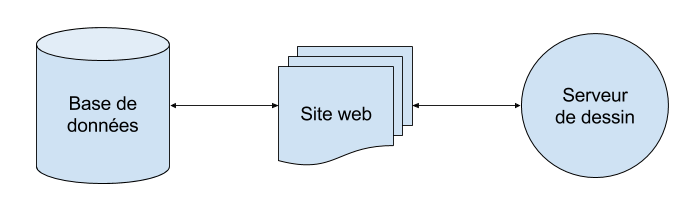
\includegraphics[width=0.8\textwidth]{sketcher_global_structure.png}
\end{center}

La base de données n'est accessible que par le site web, doté d'une API type REST permettant au serveur de dessin de lui passer des requêtes.

\subsection{Serveur Web}
Le site web est développé avec le framework Symfony 3 et utilise une base de données MariaDB.

Il joue les rôles d'interface utilisateur et de gestionnaire de base de données.

\section{Conclusion}
La création de cette application nous a permis de découvrir le framework Symfony 3 ainsi que la technologie des WebSockets. L'utilisation du Javascript pour le développement complet de l'outil de dessin nous a appris beaucoup sur ce langage, tant côté serveur que côté client.

Le déploiement de l'application a été un défi que nous avons relevé en nous documentant sur le serveur web que nous utilisions, Apache 2.4, ce qui nous a permis d'approfondir les connaissances que nous avons acquis en cours de réseau.
\newpage
\bibliographystyle{unsrt}
\bibliography{biblio}

\end{document}
